Brugergrænsefladen er opbygget efter designmønstret \gls{MVVM}. \gls{MVVM}-mønsteret adskiller Views fra systemets Model ved at tilføje en ViewModel i mellem de to. Dette gør, at Views kan operere uafhængigt af den Model som bruges. Det gør også, at dele af brugergrænsefladen kan testes nemlig ViewModel'en. En overfladisk afbildning af \gls{MVVM}-mønsteret kan ses i figur~\ref{fig:MVVM}\footnote{Billede taget fra: https://en.wikipedia.org/wiki/Model–view–viewmodel}. Da systemet bruger \gls{WPF} og med de førnævte fordele var valget på mønstret faldet på \gls{MVVM}.

\begin{figure}[H]
\centering
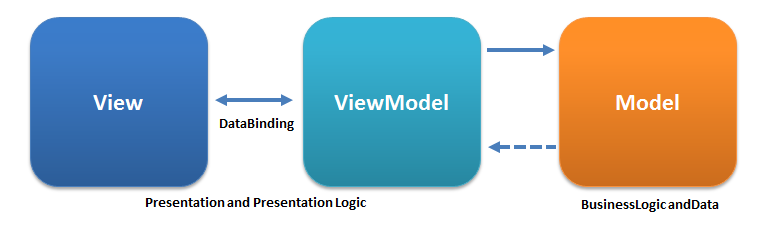
\includegraphics[width=0.8\textwidth]{N+1/MVVMPattern.png}
\caption{MVVM-mønsteret}
\label{fig:MVVM}
\end{figure}

Forbindelsen mellem Views og ViewModel eksisterer via DataBinding. Dvs. at Views kan forbindes via en \textit{property} i vores ViewModel. Dette gør det muligt at deklarere et layout i \gls{XAML}, men at holde alt programlogikken i ViewModel's.

\logicalview{0.85}{CLASS}{GUI}{pakken GUI}

Når applikationen starter vil der blive oprettet et \texttt{MainWindow}, som har en DataContext, der peger på \texttt{MainViewModel}. Dette illustreres i \ref{fig:GUI_CLASS} med et klassediagram. I \texttt{MainWindow}'s \gls{XAML} kode er de ViewModel's, som oprettes i \texttt{MainViewModel}, deklareret. Det gør at de Views, som er bundet til de deklarerede ViewModels i \texttt{App.xaml}, vil blive vist i vinduet.

\logicalview{0.85}{CLASS}{Views}{pakken Views i GUI}

På figur~\ref{fig:Views_CLASS} kan bindingerne mellem View og ViewModel ses. Det vil sige at de bindinger eller \textit{Bindings}, som sker i \gls{XAML} koden binder ned i den pågældende model. Mønsteret gør, at man ikke behøves at have meget \textit{Code Behind}. Ansvaret kan i stedet gives videre til ViewModel's.

\logicalview{0.85}{CLASS}{ViewModels}{pakken ViewModels i GUI}

På figur~\ref{fig:ViewModels_CLASS} kan der ses et klassediagram over de ViewModels, som eksisterer i kassesystemet. På figuren er \texttt{MainViewModel} systemets ''Hoved''-ViewModel. \texttt{MainViewModel} står for at oprette alle de andre ViewModels og de dertil tilhørende Views. Der findes hovedsagligt tre specialiserede ViewModels:
\begin{itemize}
	\item \texttt{SalesViewModel}: Skal håndtere tilføjelse af produkter, betaling og annullere en ordre.
	\item \texttt{TabViewModel}: Skal håndtere produktgrupperne, hvor varene i de valgte gruppe bliver vist, som knapper på brugergrænsefladen.
	\item \texttt{NumpadViewModel}: Skal håndtere de nummererede taster eller det numpad, som findes på brugergrænsefladen.
\end{itemize}

En anden fordel ved at have brugt MVVM er at mange af elementerene i GUI'en er dynamisk oprettede. I \texttt{TabView} er alle knapper dynamisk oprettede både "Tabs" og "Produkt" knapper. 
Det er her \texttt{TabViewModel} er ansvarlig for at indhente den data der skal bruges for at lave \texttt{TabView}. Det eneste der er i \texttt{XAML} for \texttt{TabView} er hvordan opsætningen skal være.
I forhold til \texttt{SalesView} er den liste af produkter der er ved at bliver solgt også lavet dynamisk og blive løbende opdateret.

\logicalview{0.85}{CLASS}{Dialogs}{pakken Dialogs i GUI}

Dialogerne i brugergrænsefladerne bruges, når der er en handling, som kræver brugerens opmærksomhed. Dialogerne kommer f.eks. når der skal vælges en betalingsmetode, eller når kassen skal afstemmes. På figur~\ref{fig:Dialogs_CLASS} kan følgende klasser ses:
\begin{itemize}
	\item \textbf{PaymentDialog}: Skal håndtere betaling af ordre.
	\item \textbf{BalanceDialog}: Skal håndtere kasse afstemning.
\end{itemize}